% !TEX TS-program = pdflatex
% !TEX encoding = UTF-8 Unicode

% This is a simple template for a LaTeX document using the "article" class.
% See "book", "report", "letter" for other types of document.

\documentclass[11pt]{article} % use larger type; default would be 10pt

\usepackage[utf8]{inputenc} % set input encoding (not needed with XeLaTeX)

%%% Examples of Article customizations
% These packages are optional, depending whether you want the features they provide.
% See the LaTeX Companion or other references for full information.

%%% PAGE DIMENSIONS
\usepackage{geometry} % to change the page dimensions
\geometry{a4paper} % or letterpaper (US) or a5paper or....
\geometry{margin=1in} % for example, change the margins to 2 inches all round
% \geometry{landscape} % set up the page for landscape
%   read geometry.pdf for detailed page layout information

\usepackage{graphicx} % support the \includegraphics command and options

% \usepackage[parfill]{parskip} % Activate to begin paragraphs with an empty line rather than an indent
\usepackage{amssymb}
\usepackage{amsmath}
%%% PACKAGES
\usepackage{booktabs} % for much better looking tables
\usepackage{array} % for better arrays (eg matrices) in maths
\usepackage{paralist} % very flexible & customisable lists (eg. enumerate/itemize, etc.)
\usepackage{verbatim} % adds environment for commenting out blocks of text & for better verbatim
\usepackage{subfig} % make it possible to include more than one captioned figure/table in a single float
% These packages are all incorporated in the memoir class to one degree or another...

%%% HEADERS & FOOTERS
\usepackage{fancyhdr} % This should be set AFTER setting up the page geometry
\pagestyle{fancy} % options: empty , plain , fancy
\renewcommand{\headrulewidth}{0pt} % customise the layout...
\lhead{}\chead{}\rhead{}
\lfoot{}\cfoot{\thepage}\rfoot{}

%%% SECTION TITLE APPEARANCE
\usepackage{sectsty}
\allsectionsfont{\sffamily\mdseries\upshape} % (See the fntguide.pdf for font help)
% (This matches ConTeXt defaults)

%%% ToC (table of contents) APPEARANCE
\usepackage[nottoc,notlof,notlot]{tocbibind} % Put the bibliography in the ToC
\usepackage[titles,subfigure]{tocloft} % Alter the style of the Table of Contents
\usepackage{bbm}
\usepackage{endnotes}

\renewcommand{\cftsecfont}{\rmfamily\mdseries\upshape}
\renewcommand{\cftsecpagefont}{\rmfamily\mdseries\upshape} % No bold!
\DeclareMathOperator*{\argmax}{arg\,max}
\DeclareMathOperator*{\argmin}{arg\,min}

\usepackage{graphicx}
\graphicspath{ {./pings/} }

\newcount\colveccount
\newcommand*\colvec[1]{
        \global\colveccount#1
        \begin{pmatrix}
        \colvecnext
}
\def\colvecnext#1{
        #1
        \global\advance\colveccount-1
        \ifnum\colveccount>0
                \\
                \expandafter\colvecnext
        \else
                \end{pmatrix}
        \fi
}

\newcommand{\norm}[1]{\left\lVert#1\right\rVert}

\title{Computational Problem Set 2}
\author{Michael B. Nattinger, Sarah J. Bass, Xinxin Hu}

\begin{document}
\maketitle

\section{Enforceable insurance markets}
With enforceable insurance markets we will have complete markets. We will solve for the Arrow-Debreu equilibrium. With no initial asset holdings, consumption for all households will be equilized in all periods. I assume trading takes place before the realization of initial states, and denote by $P_e,P_u$ the invariant distribution over employment status of the population:
\begin{align*}
V = &\max_{\{c_t^i\}_{t=0}^{\infty}} \beta^t u(c_t^i) \\
&\text{s.t.} \sum_{t=0}^{\infty} q_t c_t^i \leq \sum_{t=0}^{\infty}q_t(1*P_{e} + 0.5*P_{u})
\end{align*}
Taking first order conditions,
\begin{align*}
\beta^t u'(c_t^i) &= \lambda q_t \\
\Rightarrow u'(c_t^i) &= u'(c_t^j)\\
\Rightarrow c_t^i &= \tilde{c} := P_e + 0.5P_u \\
\Rightarrow u'(c_t^i) q_{t+1} &= \beta u'(c_{t+1}^i) q_{t} \\
\Rightarrow q_{t+1} &= \beta q_t.
\end{align*}
Normalizing $q_0 = 1, q_t = \beta^t$. Therefore, our prices of the consumption good in each period are $q_t = \beta$, and households have perfect risk sharing and each household consumes $c_t^i = \tilde{c}$ in each period.
\section{Incomplete markets}
Parts 1, 2, and 3 have been implemented by Michael in Fortran and by Sarah in Julia. The Fortran code uses the following iterated grid search specification, a similar method to bisection, by which the asset market clears to within tolerance in 7.6 seconds:
\begin{enumerate}
\item Select $q_{min}, q_{max}$ such that the asset market is sure to clear for some $q \in (q_{min},q_{max})$.
\item Partition $(q_{min},q_{max})$ into $n_{partition}\geq 3$ equal subintervals of length $\Delta = (q_{max}-q_{min})/n_{partition}$ by sampling $q_{guess}$ at the $n-1$ points in-between each interval.
\item Calculate the excess demand at each $q_{guess}$. If any $q_{guess}$ clears the market to within tolerance, break search and return that $q_{guess}$. If not, choose $\hat{q}_{guess} = \argmin_{q_{guess}} |ED(q_{guess})|$ where $ED(q)$ is the excess demand function.
\item Center the next search region at $\hat{q}_{guess}$ by updating $q_{min} = \hat{q}_{guess} - \Delta, q_{max} = \hat{q}_{guess} + \Delta$.
\item Return to step 2 until the maximum number of iterations is reached. Note that, for $n_{partition}$ even then $\hat{q}_{guess}$ will be a $q_{guess}$ on the next iteration, so excess demand does not need to be recalculated in the next iteration.
\end{enumerate}

I chose initial $q_{min} = \beta$, $q_{max} = 1$, and $n_{partition} = 4$. This results in only needing to calculate excess demand at $2$ guesses of $q$ in each iteration after the first iteration. The market clears to within a tolerance of $10^{-3}$ in the fourteenth iteration of this procedure, after only 29 guesses of $q$. I chose this method as it is significantly more stable in terms of tolerance clearing than pure bisection: as the initial width of the grid increases, increasing $n_{partition}$ appropriately ensures that the procedure will still find the appropriate minimum. For example, with an 'uninformed' initial guess of $q_{min}=0.5,q_{max} = 2$ (note $\beta/0.5>1$ which we know makes $0.5$ unlikely to clear the market, and $q=2$ implies the real interest rate is $-50\%$, which seems very unlikely) we can still converge to the same equilibrium by increasing $n_{partition}$ from $4$ to $10$. The cost of this poor choice of $q_{min},q_{max}$ is purely computational speed: convergence occurs after 37.5 seconds, after 72 iterations of q. The combination of stability and speed of this iterated grid search makes it a strong candidate for this application.

Answers to part 4 are below:

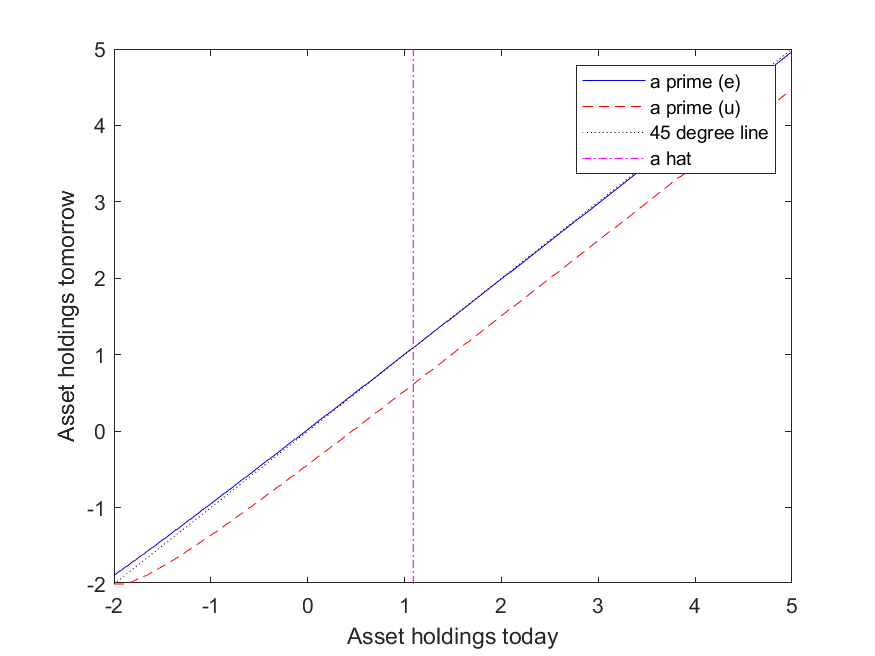
\includegraphics{aprime}

I converge to an equilibrium bond price of $q = 0.99427$. Note this is very close to the complete markets implied (inverse) gross interest rate of $\beta$, satisfies that $\beta/q < 1$, and implies a real interest rate of $r = q^{-1} - 1 = 0.0057 = 0.57\%$. 

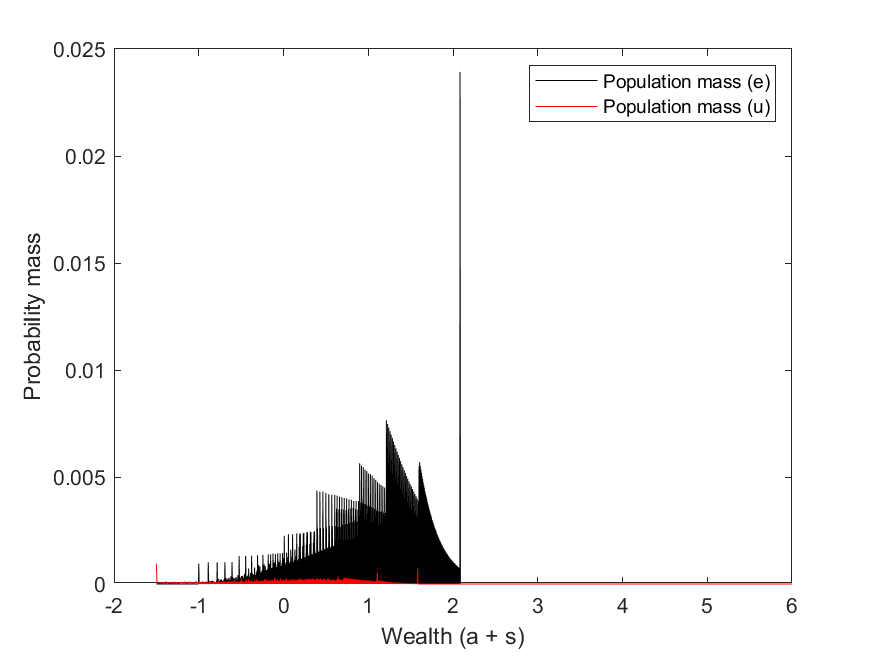
\includegraphics{wealth}

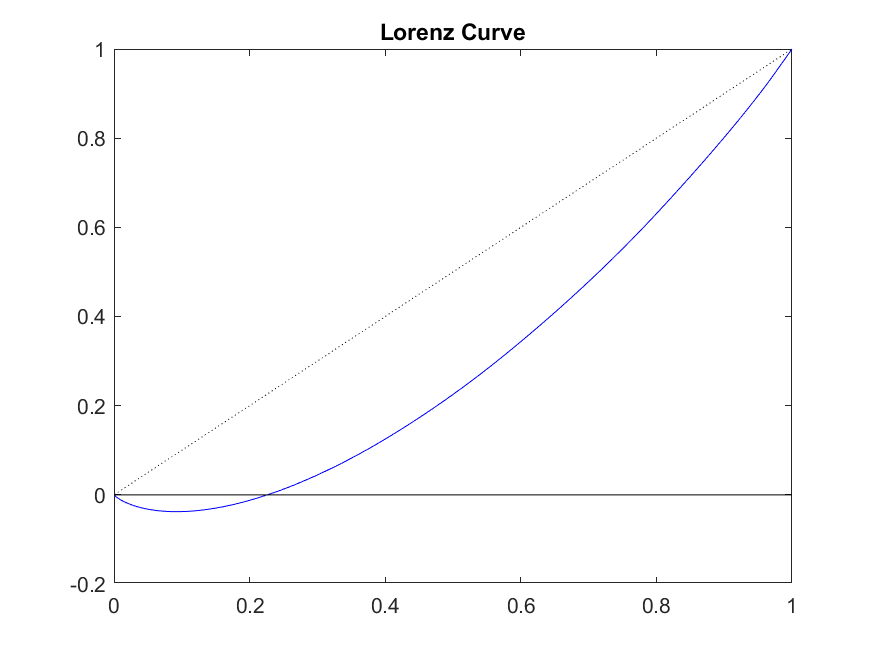
\includegraphics{lorenz}

The gini index for our economy is computed as the numerical integral of the difference between the $45$ degree line between $0,1$ and the Lorenz curve, divided by the area under the $45$ degree line. The computed gini index is $0.3845$. The true gini value for the US in 2019 was $0.48$, so our model features less inequality than we see in the data. This is also apparent from the Lorenz curve, as relative to the the data the model-implied Lorenz curve is above that of the US from the 0.3 quantile through 1. It is not above for all quantiles as many of the households in the model have negative wealth.
\section{Welfare gains}

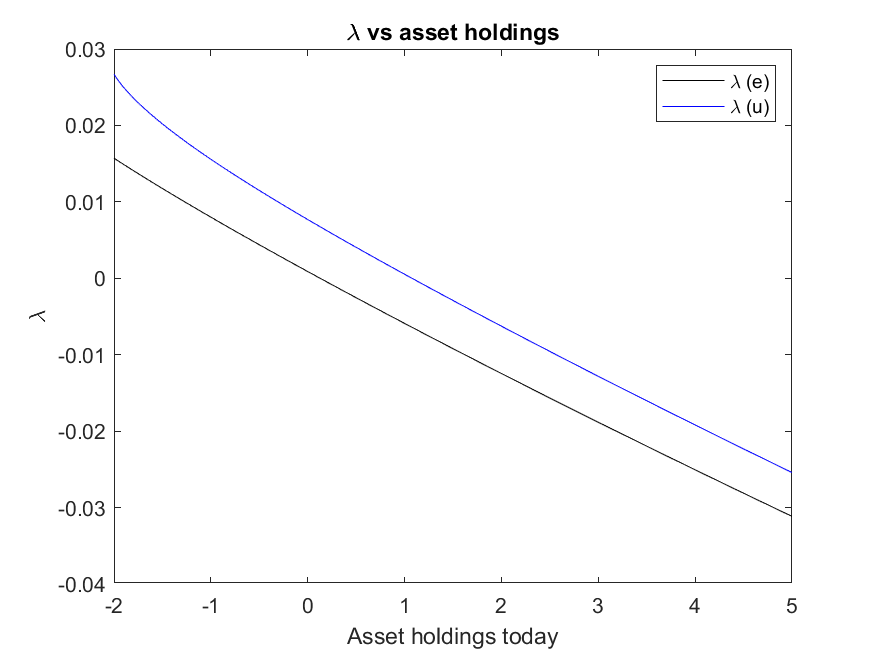
\includegraphics{lambda}

For asset holdings $\in [-2,\hat{a}]$ we can see that $\lambda$ is only above zero for the unemployed and for the relatively poor employed. Despite this, we will see that there would be societal benefits (due to convexity of the utility function) of transitioning to the planner's solution.

$W^{FB} = \frac{u(\tilde{c})}{1-\beta} = -4.2525$. $W^{INC} = -4.4557$. $WG = 0.0014$. The fraction of the market in favor of changing to complete markets is $0.5407$, or $54.07\%$.


\end{document}
